\documentclass[12pt]{report}
\usepackage[T1]{fontenc}
\usepackage[utf8]{inputenc}
\usepackage{caption}
\usepackage{adjustbox}
\usepackage{graphicx}
\usepackage{amsmath,amssymb,amsfonts}
\usepackage{txfonts}
\usepackage{listings}
\usepackage{float}
\usepackage{color}
\usepackage{xcolor}
\usepackage{enumitem}
\graphicspath{{images/}}
\renewcommand{\chaptername}{Rozdział}
\renewcommand{\contentsname}{Spis treści}
\renewcommand{\figurename}{Rysunek}
\renewcommand{\listfigurename}{Spis rysunków}
\renewcommand{\bibname}{Bibliografia}
\newtheorem{definition}{Definicja}
\newtheorem{example}{Przykład}[chapter]
\setlength{\textwidth}{14cm}
\setlength{\textheight}{20cm}
\lstdefinelanguage{JavaScript}{
  keywords={typeof, new, true, false, catch, function, return, null, catch, switch, var, if, in, while, do, else, case, break},
  keywordstyle=\color{blue}\bfseries,
  ndkeywords={class, export, boolean, throw, implements, import, this},
  ndkeywordstyle=\color{darkgray}\bfseries,
  identifierstyle=\color{black},
  sensitive=false,
  comment=[l]{//},
  morecomment=[s]{/*}{*/},
  commentstyle=\color{purple}\ttfamily,
  stringstyle=\color{red}\ttfamily,
  morestring=[b]',
  morestring=[b]"
}
\lstset{
   language=JavaScript,
   backgroundcolor=\color{lightgray},
   extendedchars=true,
   basicstyle=\footnotesize\ttfamily,
   showstringspaces=false,
   showspaces=false,
   numbers=left,
   numberstyle=\footnotesize,
   numbersep=9pt,
   tabsize=2,
   breaklines=true,
   showtabs=false,
   captionpos=b
}
\lstdefinelanguage{XML}
{
  morestring=[b]",
  morestring=[s]{>}{<},
  morecomment=[s]{<?}{?>},
  stringstyle=\color{black},
  identifierstyle=\color{blue},
  keywordstyle=\color{cyan},
  morekeywords={xmlns,version,type}% list your attributes here
}
\lstset{
  basicstyle=\ttfamily,
  columns=fullflexible,
  showstringspaces=false,
  commentstyle=\color{gray}\upshape
}
\colorlet{punct}{red!60!black}
\definecolor{background}{HTML}{EEEEEE}
\definecolor{lightgray}{rgb}{.9,.9,.9}
\definecolor{darkgray}{rgb}{.4,.4,.4}
\definecolor{purple}{rgb}{0.65, 0.12, 0.82}
\definecolor{delim}{RGB}{20,105,176}
\colorlet{numb}{magenta!60!black}
\lstdefinelanguage{json}{
    basicstyle=\normalfont\ttfamily,
    numbers=left,
    numberstyle=\scriptsize,
    stepnumber=1,
    numbersep=8pt,
    showstringspaces=false,
    breaklines=true,
    frame=lines,
    backgroundcolor=\color{background},
    literate=
     *{0}{{{\color{numb}0}}}{1}
      {1}{{{\color{numb}1}}}{1}
      {2}{{{\color{numb}2}}}{1}
      {3}{{{\color{numb}3}}}{1}
      {4}{{{\color{numb}4}}}{1}
      {5}{{{\color{numb}5}}}{1}
      {6}{{{\color{numb}6}}}{1}
      {7}{{{\color{numb}7}}}{1}
      {8}{{{\color{numb}8}}}{1}
      {9}{{{\color{numb}9}}}{1}
      {:}{{{\color{punct}{:}}}}{1}
      {,}{{{\color{punct}{,}}}}{1}
      {\{}{{{\color{delim}{\{}}}}{1}
      {\}}{{{\color{delim}{\}}}}}{1}
      {[}{{{\color{delim}{[}}}}{1}
      {]}{{{\color{delim}{]}}}}{1},
}

\begin{document}

\tableofcontents

\chapter{Wstęp}

  \section{Cel pracy}
  Celem pracy jest przedstawienie różnic, podobieństw oraz wspólnych konceptów między wybranymi frameworkami technologii Node.js. 
  Od okresu jej ukazania się powstało wiele narzędzi ułatwiających oraz poprawiających jakość procesu deweloperskiego. 
  Niektóre z nich skupiają się na usprawnianiu podobnych, pokrewnych lub identycznych przypadków użycia.
  Aby unkinąc nie trafnego wdrożenia wybranego narzędzia w opracowywany projekt, należy rozumieć kiedy wybrana metoda sprawdzi się najlepiej, a kiedy warto zastosować inne rozwiązanie.
  Nawet w przypdaku użycia tego samego języka programowania przeniesienie aplikacji pomiędzy frameworkami może być kosztownym oraz czasochłonnym przedsiemwzięciem.
  Z tego powodu powstała potrzeba zakreślenia, które wyjście najlepiej sprawdza się dla określonego projektu lub jego części.
  W pracy zostały zawarte kryteria wyboru technologii, specyfikacje ocenianych parametrów, analiza frameworków oraz podsumowanie przeprowadzonych badań.


  \section{Przeznaczenie technologii Node.js}
  Node.js jest cross-platformowym, działającym niezależnie od środowiska językiem programowania, napisanym w językach c/c++ oraz javascript, wydanym 27 marca 2009 roku, zaprojektowanym przez Ryana Dahla.
  Początkowym przeznaczeniem technologii było tworzenie serwerów i narzędzi sieciowych, działających po stronie serwera, lecz wraz z jej rozpowszechnianiem się możliwości te znacznie się poszerzyły oferując wytwarzanie między innymi aplikacji desktopowych (electron), mobilnych (react native, cordova) lub rozwiązań embedded (onoff).
  Przed jej powstaniem powstaniem kod w języku javascript był wykonywany głównie przez przeglądarkę internetową po stronie klienta, co pozwalało na bezproblemową manipulację kodem źródłowym strony przez użytkownika, dając możliwość wykonywania złośliwych skryptów, naruszenie bezpieczeństwa baz danych lub uzyskania dostępu do chronionych zasobów servera.
  Środowisko Node.js może działać niezależnie od środowiska uruchomieniowego.
  Jest ono zgodne z wieloma systemami operacyjnymi jak  Linux, macOS, Microsoft Windows, NonStop, czy serwerami Unix.
  Język ten cieszy się dużą popularnością oraz pozytywnym odbiorem wśród użytkowników, dzięki czemu, mimo względnie krótkiego okresu życia środowiska, zaowocowało ogromną ilością projektów open-source, tysiącami członków należących do społeczności okołojęzykowej oraz powstaniem wydarzeń poruszających tematy okołośrodowiskowe, takimi jak NodeConf, Node Interactive lub Node Summit.
  Obecnie wiele największych firm korzysta z serwerów napisanych w języku Node.js.
  Ich przykładami są między innymi Groupon, IBM, Linkedln, Microsoft, Netflix, PayPal, Yahoo.
  Najpopularniejszymi API wspierającymi edycję oraz debugowanie kodu Node.js są Atom, Visual Studio Code czy WebStorm.
  \newline Node.js zalecany jest do tworzenia aplikacji: 

  \begin{itemize}
    \item z dużą liczbą operacji wejścia/wyjścia,
    \item strumieniowania danych np. video, 
    \item Single Page Applications (SPA),
    \item udostępniających API w formacie JSON,
    \item z intensywną wymianą danych w czasie rzeczywistym na wielu urządzeniach, np. portalach społecznościowych.
  \end{itemize} 

  Ponieważ jest on szybki i lekki, może być stosowany do pisania między innymi bramki API.
  API to skrót od Application Programming Interface; opisuje, jak poszczególne elementy lub warstwy oprogramowania powinny się komunikować.
  W praktyce to najczęściej biblioteka oferująca metody, które umożliwiają realizację określonych zadań.
  Node.js pozwala na zoptymalizowanie pracy oraz uzyskanie skalowalności dzięki asynchronicznemu przetwarzaniu danych dostarczanych do aplikacji, w związku z czym idealnie nadaje się do obsługi komunikacji wymagającej pracy w czasie rzeczywistym. 
  Przeciwnie do języków gdzie program jest wykonywany linia po linii, funkcje napisane w Node.js nie wykonują się synchronicznie, korzystając z tak zwanych wywołań zwrotnych (ang. callback).
  Dzięki temu nie powstaje problem blokowania określonych funkcjonalności programu w czasie pracy innych, niezależnych jego części.
  Przy pomocy wywołań zwrotnych możemy zapewnić zasygnalizowanie uzyskanych wyników lub zwrócenie, bądź obsługę błędu powstałego w czasie działania bloku kodu.

  \section{Potrzeba rozwoju narzędzi deweloperskich}
  Nieustany rozwój lub powstawanie nowych narzędzi powoduję ciągłą potrzebe nauki na inżynierach.
  Bez przerwy pojawiają się nowe rozwiązania, które sprawiają że dotychczasowe odchodzą w nie pamięć lub ich użycie kojarzy się z zacofaniem oraz pozostaniem w tyle.
  Absolutnie nie powinno uważać się tego zjawisko za negatywne.
  Powstanie nowego narzędzia jest inicjowane przez kogoś kto zauważył pewną regularność danego przypadku użycia.
  Nie tylko sprawia to że mniej czasu należy poświęcić na uzyskanie pewnej określonej funkcjonalności, ale przede wszystkim daje możliwość skorzystania z wiedzy i praktyk wielu osób mających doświadczenie w danej dziedzinie, które napotykały dokładnie te same problemy.
  Korzystamy wówczas nie tylko z najlepszych praktyk programistycznych, ale także zapewniamy sobie dostęp do przetestowanych sprawdzonych metod.
  Bardzo żadkim zjawiskiem jest natrafienie na jakąmś nieścisłość, wywołującą niepoprawne działanie własnego kodu.
  Nawet w takich przypadkach błedy te są bardzo szybko poprawiane przez specjalistów, którzy zdejmują z nas odpowiedzialność od utrzymaniu pewnego kodu.
  Rozwiązania używane globalnie zapewniają róznież szybsze wdrażanie się w nowe projekty.
  Nowe osoby zostają odciążone od poznawania części aplikacji, ponieważ korzystały już z tych samych rozwiązań.
  Należy natomiast upewnić się czy wykorzystując dane gotowe narzędzie nie dołączamy do istniejącego projektu mnóstwa innych, zbędnych zasobów.
  Wiele funkcji dostarczanych nie jest wykorzystywanych i może zostać nie potrzebnie zawarta w końcowym produkcie.
  W celu tego uniknięcia możemy skorzystać z wybranych bundlerów (np. webpack), które odrzucą nieużywane części kodu minimalizując rozmiar aplikacji.

\chapter{Kryteria wyboru freameworkow}

  \section{Poszukiwanie}
  Wszystkie aktualnie liczące się frameworki odnośnie technologi Node.js możemy znaleźć na stronie "http://nodeframework.com/".
  Strona jest prowadzona przez społeczeństwo deweloperów.
  Może zostać zaktualizowana poprzez zaakceptowanie przez twórce projektu Azat Mardan'a merge requesta w serwisie github. 
  Oznacza to, że strona posiada aktualne infromacje na temat używanych na świecie rozwiązań.
  W celu wybrania konkretnych frameworków do badań warto zwrócić uwagę na pare konkretnych kwesti.
  Analizowane narzędzie z pewnością powinno być używane przez deweloperów na liniach produkcyjnych.
  Gwarantuje nam to że jest to narzędzie sprawdzone w bezpośrednium użyciu.
  Powinno cieszyć się ono równierz względnie dużą popularnością, aby upewnić się że radzi sobie przy różnych wielkościach projektów, w różnym stadium zaawansowania, oraz różnym poziomie skomplikowania.
  Najlepiejby było aby framework był wciaż rozwijany, ponieważ znaczyło by to że jego funkcjonalność jest wciąż poszerzana oraz że nie jest przestażały.
  Parametry te możemy sprawdzić wchodząc na repozytoria frameworków.
  Przykładowo możemy sprawdzić, że locomotive posiada tylko 868 gwiazdek oraz że ostatnia aktualizacjia była 17 października 2017 roku (dane na dzień 06.06.2018), więc możemy wywnioskować że nie cieszy się on dużą popularnością oraz że nie jest już odświeżany.

  \begin{figure}[!hb]
    \centering
    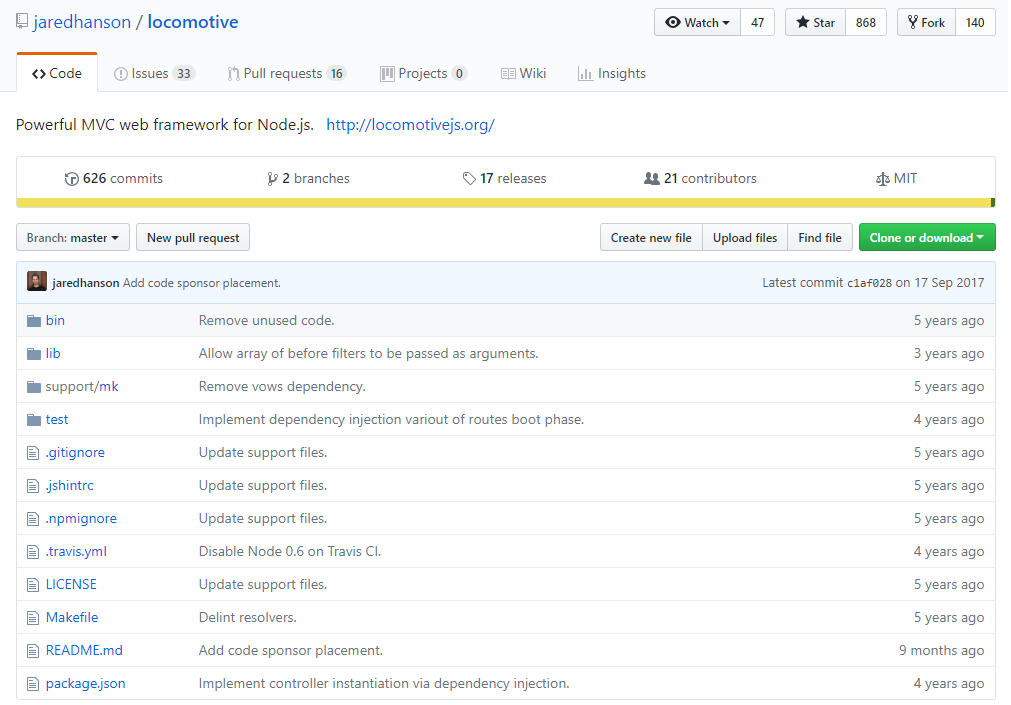
\includegraphics[width=\textwidth,height=\textheight,keepaspectratio]{locomotive.png} 
    \caption{Strona projektu locomotive w serwisie github, źródło: https://github.com/jaredhanson/locomotive/}
  \end{figure}

  Dla porównania framework koa posiada 21568 gwiazdek oraz był aktualizowany przed 9-cioma godzinami (dane na dzień 06.06.2018). Możemy wieć założyć że jest wciąż popularny oraz utrzymywany.

  \begin{figure}[!hb]
    \centering
    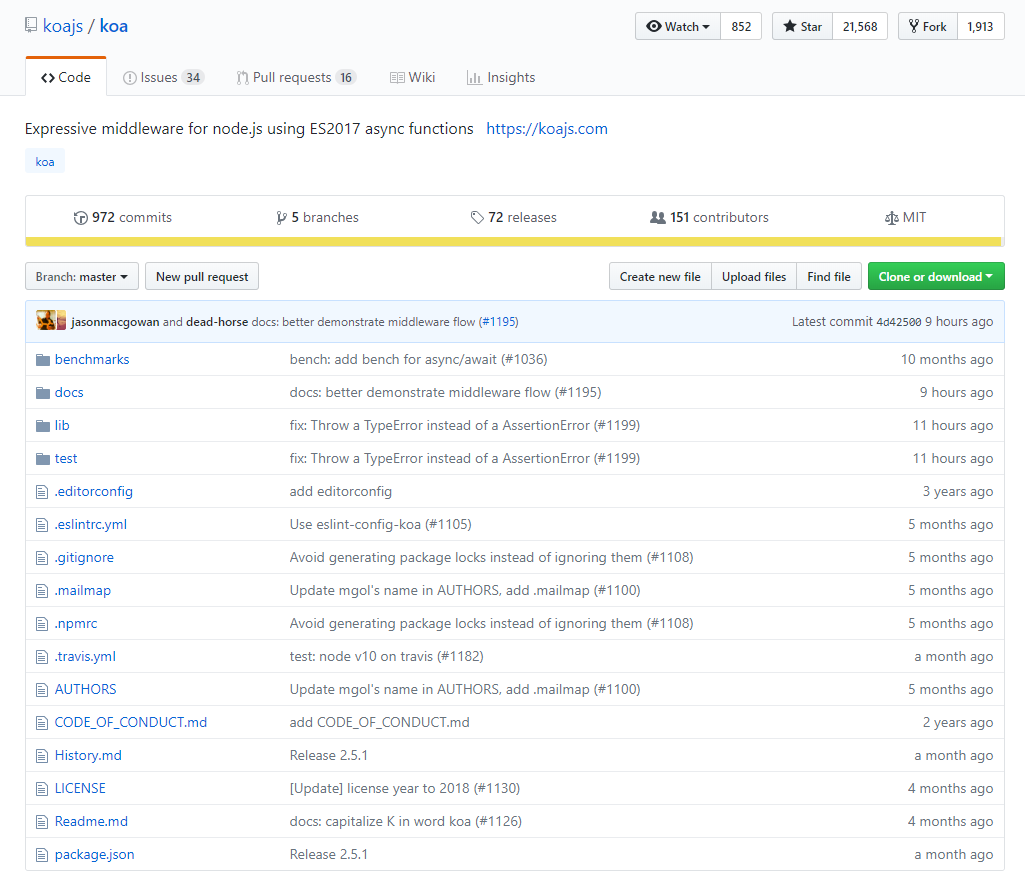
\includegraphics[width=\textwidth,height=\textheight,keepaspectratio]{koa.png} 
    \caption{Strona projektu koa w serwisie github, źródło: https://github.com/koajs/koa/}
  \end{figure}

  \section{Wybrane frameworki}

  Ilość dostępnych narzędzi nie pozwala niestety na porównanie wszystkich rozwiązań.
  W związku z czym zdecydowałem się przeanalizować w pracy 3 wybrane - express, sails oraz meteor.

  \newline
  Express wybrałem ze wzgłedu na jego ogromną popularność. 
  Repozytorium projektu posiada prawie 40000 gwiazdek w serwisie github oraz jest najpopularniejszy ze wszystkich frameworków w serwisie stackoverflow (dane na dzień 06.06.2018).
  Ze wszystkich konkurencyjnych rozwiązań jest najpopularniej wymienianą technologią w ofertach pracy.

  \newline
  Sails...

  \newline
  Meteor...
  
  \section{Alternatywne rozwiązania}



\chapter{Kryteria oceny}

  \section{Skala oraz wagi ocen}
  - oceny od 1 do 3 1 - wogole nie wspiera trzeba uzyc osobnego narzedzia / wolne / wymaga duzo pracy czym wiecej kodu tym ciezej / cieszkie opisy przyswajanie
  2 - wspiera czesciowo jednak trzeba skonfiguraowac narzedzie / srednie / wymaga noramlnie kodu. nie rosnie z czasem / ok oopisy zrozuumiale
  3 - w pelni wspiera lub minimalny efort w celu dzialania / bardzo predko / czym wiecej juz mam napisane tym mniej mam pisac / super dokumetacja wsparcie testowe kody i zloto
  do tego rozne wagi

  \section{Parametry}
  \subsection{Rozmiar}
  \subsection{Warstwa widoku}
  \subsection{Warstwa bazy danych}
  \subsection{Benchmark}
    - szybkosc przy rownoleglych zapytaniach
    - szybkosc przy kolejnych zapytaniach
  \subsection{Rozszerzalność}
  \subsection{Testowanie}
  \subsection{Popularność}
  \subsection{Dokumentacjia}
    - przyswajalnosc
    - dostepnosc
    - szczegolowosc / wielkosc bo nie wystrcz ywiekosc moze miec malo funkcji ale umiec wszystko
  \subsection{Wielkość kodu}
  \subsection{Prog wejscia}
  \subsection{Podsumowanie}
    tabelka co ile wagi

\chapter{Opis wybranych rozwiązań}

  \section{Sails}

  \section{ExpressJS}

  \section{Meteor}

\chapter{Analiza porównawcza}
- dla kazdej technologi o kazdym kryterium oceny

\chapter{Podsumowanie}

  \subsection{Podsumowanie ocen}

  \subsection{Wskazywane zastosowania}

\addcontentsline{toc}{chapter}{Bibliografia} 
\begin{thebibliography}{99}
  \bibitem{Brown}
  E. Brown
  \textit{"Web Development with Node and Express", 2014}

  \bibitem{Mardan}
  Azat Mardan
  \textit{"Express.js Guide: The Comprehensive Book on Express.js", 2016}

  \bibitem{StrongLoop}
  StrongLoop
  \textit{dokumentacja Express, 2017, źródło: https://expressjs.com/en/4x/api.html}

  \bibitem{McNeil&Nathan}
  Mike McNeil, Irl Natha
  \textit{"Sails.js in Action", 2017}

  \bibitem{Shahid}
  Shahid Shaikh
  \textit{"Sails.js Essentials", 2016}

  \bibitem{McNeil}
  Mike McNeil
  \textit{dokumentacja Sails, 2017, źródło: https://sailsjs.com/documentation/reference}

  \bibitem{Strack}
  Isaac Strack
  \textit{"Getting Started with Meteor JavaScript Framework", 2012}

  \bibitem{Vogelsteller&Strack&Reyna}
  Fabian Vogelsteller, Isaac Strack, Marcelo Reyna
  \textit{"Meteor: Full-Stack Web Application Development", 2016}

  \bibitem{MDG}
  Meteor Development Group
  \textit{dokumentacja Meteor API, 2017, źródło: https://docs.meteor.com/\#/full/}

  \bibitem{Onodi}
  Node.js Foundation
  \textit{dokumentacja języka programowania Node.js, 2017, źródło: https://nodejs.org/en/docs/}

  \bibitem{Wolff}
  Eberhard Wolff
  \textit{"Microservices: Flexible Software Architecture", 2016}

  \bibitem{Zeidman}
  Bob Zeidman
  \textit{"The Software IP Detective's Handbook: Measurement, Comparison, and Infringement Detection", rok}

\end{thebibliography}

\addcontentsline{toc}{chapter}{Spis rysunków} 
\listoffigures

\end{document}